\documentclass[12pt]{article}
\usepackage{amsmath}
\usepackage{sectsty}
\usepackage{graphicx}
\usepackage{amssymb}
\usepackage{tikz}
\usepackage{tkz-euclide}
\usepackage{xcolor}
\usepackage{soul}
\renewcommand\l[0]{\lambda}

% Margins
\topmargin=-0.45in
\evensidemargin=0in
\oddsidemargin=0in
\textwidth=6.5in
\textheight=9.0in
\headsep=0.25in
\title{Finding The Equation Of A Curved Surface}
\author{AJM432}
\date{June 20, 2022}

\begin{document}
\maketitle	

\begin{figure}[htp]
    \centering
    \includegraphics[width=10cm]{curved_surface.png}
    \caption{A curved surface composed of intersecting lines}
    \vspace{4 cm}
\end{figure}

\section{Purpose}
The purpose of this paper will be to find and analyze the equation of the curve in Figure 1.

\section{Finding a General Equation for all Line Segments}
Let $g(x)$ represent the general equation of each line where $g(x)=mx+b$.
The lines begin from $(0, \l - t)$ and ends at $(t, 0)$ where $\l$ represents the bounding region of the curve.

\begin{figure} 
    \vspace{1cm}
    \begin{center}
    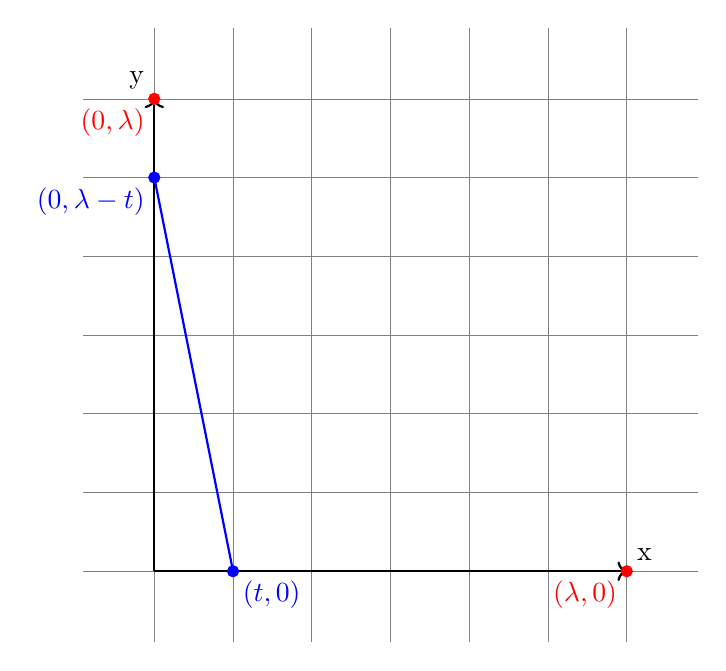
\begin{tikzpicture}
        
        \draw[step=1cm,gray,very thin] (-0.9,-0.9) grid (6.9,6.9);
        
        \draw[thick,->] (0,0) -- (6,0) node[anchor=south west] {x};
        \draw[thick,->] (0,0) -- (0,6) node[anchor=south east] {y};
        \draw[blue, thick, solid] (0, 5) -- (1,0);
        \filldraw[blue] (1,0) circle (2pt) node[anchor=north west]{$(t, 0)$}; 
        \filldraw[blue] (0,5) circle (2pt) node[anchor=north east]{$(0, \l-t)$}; 
        \filldraw[red] (0,6) circle (2pt) node[anchor=north east]{$(0, \l)$}; 
        \filldraw[red] (6,0) circle (2pt) node[anchor=north east]{$(\l, 0)$}; 
        \vspace{1cm} 
    \end{tikzpicture}
    \caption{Labelled diagram of a single line} 
    \end{center} 
\end{figure}

$$g(0) = \l-t$$
$$\implies g(x) = mx + \l-t$$
$$g(t) = 0$$
$$0=mt + \l-t$$
$$\implies m=\frac{t-\l}{t}$$
$$\boxed{g(x) = \frac{t-\l}{t}x + \l-t}$$

\vspace{4cm}

\section{Finding the Equation of the Bounding Curve $f(x)$}

\subsection{Deriving the Tangent of a Function at any Point}
Let us recall how to find the equation of a tangent line of function at any point.
Let $T(x)$ denote the tangent line of a function $f(x)$ at $x=a$. The slope of the tangent is given by $f'(x)$. Therefore the tangent function is of the form $T(x) = f'(a)x + b$.

$$T(a) = f(a)$$
$$T(a) = a f'(a) + b$$
$$f(a) = a f'(a) + b$$
$$\implies b=f(a)- a f'(a)$$
$$\boxed{T(x)=f'(a)x + f(a)- a f'(a)}$$

\subsection{The Differential Relationship Between $g(x)$ and $f(x)$}
Now we must reverse this process and find $f(x)$.
Let $f(x)$ represent the curve created by the tangents of the intersecting lines at the curved boundary in Figure 1. In the previously derived equation $g(x)$ we see that it is the output of mapping $f(x)$ to $T(x)$. 
$$T: f \mapsto g$$

Essentially, we are solving a differential equation which satisfies the following equation where $a$ is the point of tangency and $\l$ represents the bounding region of the curve.
$$g(x) = f'(a)x + f(a) - a f'(a)$$

\subsection{Finding $f(x)$ Through a Limiting Process of Adjoining Tangents}
Let us consider the points that compose $f(x)$. These points are the result of the intersection of the lines created by altering the value of $t$ in $g(x)$ between the interval $(0, \l)$. To find $f(x)$ we need to find the intersection points for any value of $t$ in the defined interval. This intersection is our $a$ value from the tangent function definition.

\vspace{1 cm}

Let $\epsilon$ represent a small change in $x$ that will be used to find the intersection of two consecutive lines $g(x, t)$ and $g(x, t+\epsilon)$ where $g(x, t) := \dfrac{t-\l}{t}x + \l-t$. To find the intersection of these lines we will set them equal to each other.

$$g(x, t) = g(x, t+\epsilon)$$
$$\dfrac{t-\l}{t}x + \l-t = \dfrac{t+\epsilon-\l}{t+\epsilon}x + \l-t-\epsilon$$
$$x \left(\dfrac{t-\l}{t}-\dfrac{t+\epsilon-\l}{t+\epsilon}\right) = \l -t -\epsilon -\l + t$$
$$x=\dfrac{t(t+\epsilon)}{\l}$$

We have now found the x-value of the intersection of two lines whose points of tangency to $f(x)$ are separated by a distance of $\epsilon$. Now we may consider what occurs when $\epsilon$ approaches zero. We will get the exact value of $x$ at which a point of tangency occurs on $f(x)$.

$$x = \lim_{\epsilon \to 0^+} \dfrac{t(t+\epsilon)}{\l}$$
$$\boxed{x = \dfrac{t^2}{\l}}$$


Since we have found the exact value of $x$ at which the tangency occurs in terms of $t$ we can plug this result back into $g(x, t)$. However, since $f(x)$ does not depend on $t$ we must solve for $t$ in terms of $x$ to solve for $f(x)$.

$$t = \sqrt{x\l}$$

We can now transform $g(x)$ into the non-linear function $f(x)$ by a change of variables with $t$ and $x$.

$$f(x) = g \left(x, t \right) \text{ at the point of tangency } x=a$$
$$f(x)=\dfrac{t-\l}{t}x + \l - t$$

We will now substitute $t=\sqrt{x \l}$ to find $f(x)$.
$$f(x) = \dfrac{\sqrt{x\l}-\l}{\sqrt{x\l}}x + \l - \sqrt{x\l}$$
$$\boxed{f(x) = x+\l -2\sqrt{x\l}} \, x\in (0, \l)$$

\begin{figure}[htp]
    \centering
    \includegraphics[width=10 cm]{f(x).png}
    \caption{Solution Curve of $f(x)$}
\end{figure}

\vspace{5 cm}

\end{document}
